% ============================================================== QUESTION 2 (part a)
\newpage
\section*{Question 2 --- Motion or Memory?}
\addcontentsline{toc}{section}{Question 2 --- Motion or Memory?}

\noindent\textbf{Reading guide.} Tables and figures are numbered as in the handout (Table 1--6, Figure 1--6); extra material is labelled S1, S2. Unless stated otherwise, model-performance numbers are on the 1000 test videos ($9000$--$9999$), at $1\times$ with $t=1$; every learned model was trained with seeds 0 and 1 and tables report \emph{mean (seed 0, seed 1)} (per-seed rows are shown); figures and GIFs use the seed-0 model. Errors have three significant figures, scientific notation below $10^{-3}$. Code, logs and GIFs: see the repository on page 1 (\texttt{src/}, \texttt{results/}, \texttt{figures/}, \texttt{predictions/}).

\noindent\textbf{Hardware and software.} NVIDIA GeForce RTX 4060 Laptop GPU (8\,GB), 24-thread CPU, WSL2; PyTorch 2.10.0+cu128 (CUDA 12.8, cuDNN defaults, fp32 with TF32 convolutions allowed), torchvision 0.25, OpenCV 4.13, conda env \texttt{PA1\_DL}. The whole dataset (uint8) lives on the GPU. \emph{Training time} = mean wall-clock seconds per epoch over the 30 epochs (CUDA-synchronised; validation monitoring excluded); \emph{inference time} = median of five timed passes over the 1000 original test windows at batch size 32, batches already on the GPU, \texttt{model.eval()} and \texttt{torch.no\_grad()}. All models were trained one after another on the otherwise idle GPU so that times are comparable.

% ------------------------------------------------------------------ 1. Setup
\subsection*{1.\ Setup}
\begin{table}[H]\centering\small
\caption{Sanity checks of the transformation and window functions (the same functions every experiment calls). (d), (e): (frame, row, column), 0-based, for $p[7,0,10,20]=1$. For (a)--(c) \texttt{torch.equal} returned \texttt{True}.}\label{tab:t1}
\begin{tabular}{llll}\toprule
 & Check & Expected & Yours \\ \midrule
(a) & $\max|M(M(x))-x|$ & 0 & 0.0 \\
(b) & $\max|R^{4}(x)-x|$ & 0 & 0.0 \\
(c) & $\max|MRM(x)-R^{-1}(x)|$ & 0 & 0.0 \\
(d) & bright pixel of $M(p)$ (frame, row, column) & $(7,10,43)$ & $(7, 10, 43)$ \\
(e) & bright pixel of $R(p)$ (frame, row, column) & $(7,43,10)$ & $(7, 43, 10)$ \\ \midrule
(f) & $1\times$ input / target frames & 1--5 / 6--10 & 1, 2, 3, 4, 5 / 6, 7, 8, 9, 10 \\
(g) & $2\times$ input / target frames & 1, 3, 5, 7, 9 / 11, 13, 15, 17, 19 & 1, 3, 5, 7, 9 / 11, 13, 15, 17, 19 \\
(h) & $3\times$ input / target frames & 1, 4, 7, 10, 13 / 16, 19 & 1, 4, 7, 10, 13 / 16, 19 \\
\bottomrule\end{tabular}
\end{table}
Videos are split by index ($0$--$7999$ / $8000$--$8999$ / $9000$--$9999$), scaled to $[0,1]$, and windows follow eq.~(2) exactly (the same \texttt{gather\_windows} serves training, evaluation and Table~1). Symmetry $g=4m+a$ means $M^mR^a$ (rotate first, then mirror); $g^{-1}$ is implemented as ``mirror first (if $m=1$), then $R^{-a}$''.

\begin{figure}[!htbp]\centering
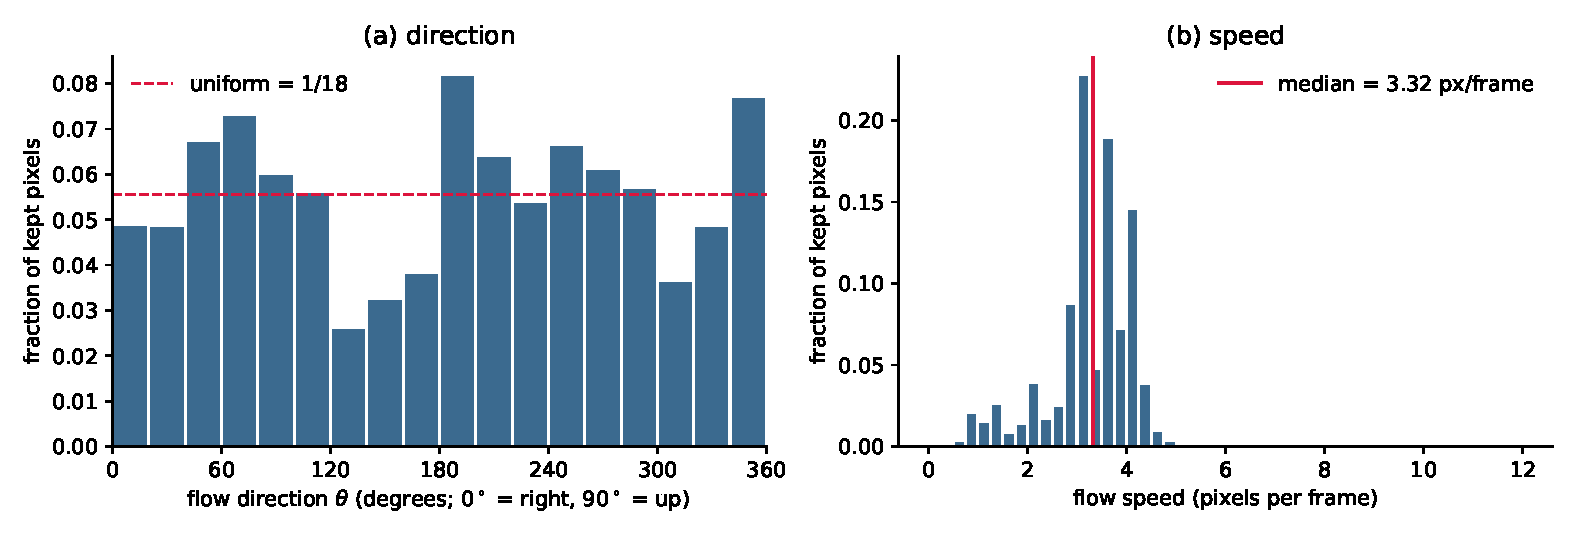
\includegraphics[width=0.97\linewidth]{fig1_flow.pdf}
\caption{Farneback optical flow on the first 50 training videos, pooled over $50\times19=950$ frame pairs; kept pixels (intensity $>0.2$ in both frames, flow magnitude $>0.5$ px): $N=103{,}050$. (a) direction $\theta=\operatorname{atan2}(-d_y,d_x)$, 18 bins of $20^\circ$ (fraction of kept pixels); the dashed line is the uniform level $1/18$. (b) speed in pixels per frame; \textbf{median speed $=3.32$ px/frame} (vertical line).}\label{fig:f1}
\end{figure}

\Q{Q2.1}{\textbf{Yes, mirrored and rotated trajectories are already familiar.} Figure~\ref{fig:f1}a is flat within sampling noise: the 18 bins lie between $0.026$ and $0.082$ around the uniform level $0.056$. This is what only 100 independent digit trajectories (50 videos $\times$ 2 digits) can produce: for 100 draws from a perfectly uniform direction law the largest relative deviation of an 18-bin histogram averages $0.88$ ($95^{\rm th}$ percentile $1.34$, Monte Carlo, 5000 draws), while we observe $0.53$. Mirroring sends $\theta\mapsto180^\circ-\theta$ and a $90^\circ$ rotation sends $\theta\mapsto\theta+90^\circ$ (4.5 bins). If every training video were mirrored, the histogram would be reflected about the vertical axis; if every video were rotated by $90^\circ$ it would be shifted by 4.5 bins; a flat histogram is unchanged by both, so the transformed directions are as common as the original ones. Quantitatively the total-variation distance between the histogram and its mirror image is $0.13$ (null mean $0.21$, $95^{\rm th}$ percentile $0.31$) and to its $90^\circ$-rotated copy $0.16$ (null $0.21$, $0.28$): no detectable asymmetry. Elastic bounces also reflect the velocity at the walls, so every trajectory visits mirror-image directions anyway. \emph{Speed:} the median is $3.32$ px/frame (inter-quartile range $3.00$--$3.89$, $5$--$95\%$: $1.41$--$4.32$; only $0.006\%$ of pixels exceed $8$ px/frame). The $2\times$ and $3\times$ videos therefore move about $6.6$ and $10.0$ px per frame \emph{between the frames the model sees} ($8.6$ and $13.0$ px for the $95^{\rm th}$-percentile speed): a range that never occurs at $1\times$. \emph{Overlap bias:} I recomputed Figure~\ref{fig:f1} after discarding every frame pair in which the two digits form one blob in either frame (443 of 950 pairs, where flow is unreliable): the median speed becomes $3.24$ px/frame, the largest relative deviation of the direction histogram from uniform $0.53$ (unchanged) and no pixel exceeds $8$ px/frame. The bias is too small to change the answer.}

\Q{Q2.2}{\begin{center}\small\begin{tabularx}{\linewidth}{@{}>{\raggedright\arraybackslash}p{2.2cm}>{\raggedright\arraybackslash}X>{\raggedright\arraybackslash}X@{}}\toprule
Transformation & Motion statistics & Digit appearance \\ \midrule
Mirror $M$ & unchanged: speeds identical, directions $\theta\to180^\circ-\theta$ (uniform $\Rightarrow$ same law) & \textbf{changed} (a mirrored 2 is not a 2) \\
Rotation $R$ & unchanged: speeds identical, $\theta\to\theta+90^\circ$ (same law) & \textbf{changed more} (stroke orientation too) \\
Speed-up $k\times$ & \textbf{changed}: displacement between seen frames $\times k$, directions unchanged & unchanged (same digits) \\ \bottomrule
\end{tabularx}\end{center}
Each transformation changes \emph{one} factor and leaves the other fixed: $M$ and $R$ change what the digits look like but keep the family of motions (a constant-velocity trajectory with elastic bounces in a square box is still valid after the symmetries of the square), while speed-up keeps the digits and changes the motion. A model that has learned \emph{how things move} should therefore be indifferent to $M$ and $R$ and should cope with $k\times$ as long as the motion is within its capacity; a failure under $M$/$R$ points to dependence on appearance, a failure under $k\times$ to unfamiliar motion or to architectural reach. That separation is what makes the three useful as a controlled experiment.}

% ------------------------------------------------------------------ 2. Baseline
\subsection*{2.\ Baseline: ConvLSTM}
Model A is implemented exactly as specified (pixel-unshuffle(4); two ConvLSTM layers, 64 hidden channels, $3\times3$ kernels, one convolution for all four gates, no peepholes; $1\times1$ conv $64\to16$, pixel-shuffle, sigmoid; 9-step free-running rollout, no teacher forcing, gradients through the fed-back predictions; states zero-initialised per video). It has \textbf{480,784} trainable parameters, as required. Training: Adam ($10^{-3}$), batch 32, 30 epochs, final-epoch weights, squared error averaged over pixels and available target frames then over videos.

\begin{table}[H]\centering\small
\caption{Test-set forecast error at $1\times$, $t=1$ (1000 test videos): per-horizon MSE, $E^{(5)}$ and trainable parameters.}\label{tab:t2}
\begin{tabular}{lrrrrrrr}\toprule
Predictor & MSE$_1$ & MSE$_2$ & MSE$_3$ & MSE$_4$ & MSE$_5$ & $E^{(5)}$ & Params \\ \midrule
Model A (mean of seeds 0, 1) & 0.0171 & 0.0203 & 0.0225 & 0.0241 & 0.0258 & 0.0220 & 480{,}784 \\
\quad seed 0 & 0.0173 & 0.0206 & 0.0228 & 0.0244 & 0.0260 & 0.0222 & 480{,}784 \\
\quad seed 1 & 0.0169 & 0.0201 & 0.0222 & 0.0239 & 0.0256 & 0.0217 & 480{,}784 \\
Blank & 0.0426 & 0.0426 & 0.0426 & 0.0425 & 0.0425 & 0.0426 & 0 \\
Copy-last & 0.0492 & 0.0604 & 0.0669 & 0.0708 & 0.0732 & 0.0641 & 0 \\
\bottomrule\end{tabular}
\end{table}
\begin{figure}[!htbp]\centering
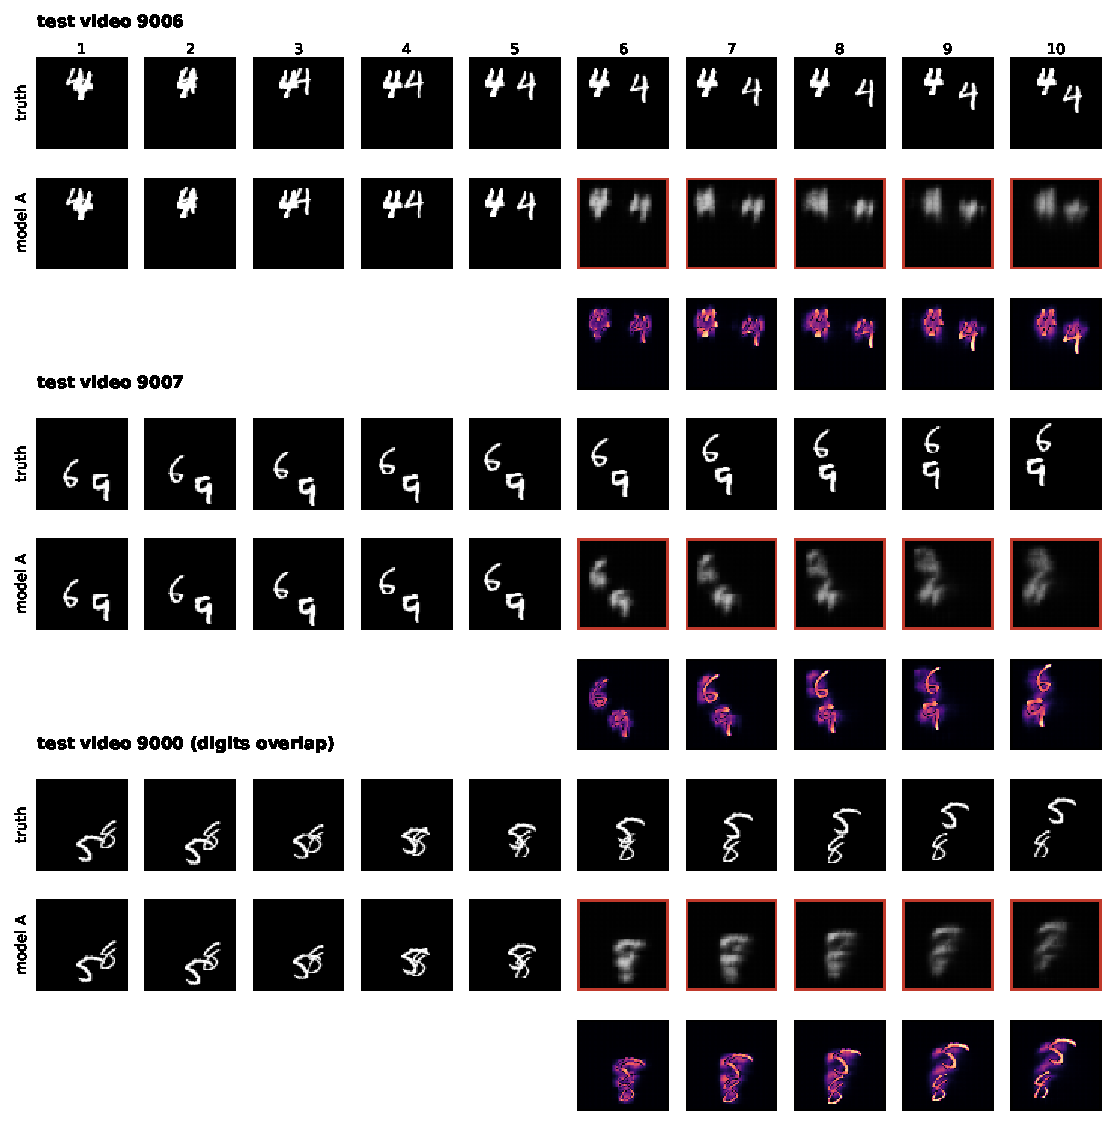
\includegraphics[width=0.86\linewidth]{fig2_predictions.pdf}
\caption{Model A (seed 0) on three test videos: 9006 and 9007 (digits never overlap in frames 6--10) and 9000 (digits overlap). For each: truth (frames 1--10), inputs 1--5 followed by the prediction of frames 6--10 (red frame), and the absolute error.}\label{fig:f2}
\end{figure}

\Q{Q2.3}{\textbf{Reach of model A $=8$ original pixels per time step.} Follow the longest path inside one step $\tau$ to the prediction $\hat x_{\tau+1}$. (i) One cell of the folded grid is 4 original pixels; a $3\times3$ convolution moves information by at most one cell, i.e.\ 4\,px. (ii) The new input $u_\tau$ is folded and enters layer~1, whose gates see a $3\times3$ neighbourhood of it ($1$ cell); layer~1's \emph{new} hidden state $h^{(1)}_\tau$ is the input of layer~2, whose $3\times3$ kernel adds one more cell ($1$ cell); the $1\times1$ output convolution, pixel-shuffle and sigmoid move nothing. Total $2$ cells $=8$\,px. (iii) The previous state $h^{(1)}_{\tau-1}$ takes the same route through layer~1's recurrent half and layer~2's input: $2$ cells; $h^{(2)}_{\tau-1}$ enters only layer~2's recurrent half: $1$ cell. The cell state $c$ is combined point-wise and moves nothing. The longest path is therefore $2\times4=\mathbf{8}$\,px, \emph{per step}; the recurrence lets state carry information further over several steps, but a digit that jumps farther than $8$\,px between two frames cannot be connected to its old position inside a single update. I checked this numerically: the gradient of one output pixel of one step with respect to $u_\tau$, $h^{(1)}_{\tau-1}$, $h^{(2)}_{\tau-1}$ is non-zero out to exactly $2$, $2$ and $1$ cells (\texttt{src/reach\_check.py}), i.e.\ $8$ px.}

\Q{Q2.4}{\textbf{Versus the references.} At $1\times$, model A (mean of seeds) has $E^{(5)}=0.0220$, against $0.0426$ for Blank ($-48\%$) and $0.0641$ for Copy-last ($-66\%$); it is better at every horizon ($\mathrm{MSE}_1$: $0.0171$ vs $0.0426$ and $0.0492$). \textbf{Error growth:} MSE rises steadily from $0.0171$ ($h{=}1$) to $0.0258$ ($h{=}5$), $+51\%$, i.e.\ about $0.0022$ per horizon, because every predicted frame is fed back and errors compound; Copy-last grows by a similar $+49\%$ ($0.0492\to0.0732$) and Blank stays flat. Even at $h{=}1$ model A is only $2.5\times$ better than Blank: Figure~\ref{fig:f2} shows that its forecasts are \emph{blurry}, at the right place but without sharp strokes, and they fade and spread with the horizon (the network hedges between possible shapes and positions). \textbf{Overlapping digits} (video 9000): the digits cross, and the forecast is a single smeared blob; the error map lights up along both digits' strokes, because the network cannot tell which stroke continues in which direction after the crossing and predicts an average of the possibilities. This is a failure of \emph{identity}, not a large increase of the average MSE: over the $586$ test videos whose digits overlap in frames 6--10, model A's $E^{(5)}$ is $0.0216$ against $0.0225$ for the other $414$ (seed-0/1 mean), since overlapping digits cover less area.}

\Q{Q2.5}{\textbf{Prediction, written before running any ``Testing the Baseline'' experiment} (verbatim from \texttt{predictions/Q2.5.md}, committed before \texttt{exp\_baseline.py} was run). \emph{Written before any Tables 3--4 or Figures 3--5 existed; I disclose that the training logs print the validation $E^{(2)}$ at $2\times$ and $3\times$, which I had seen (about 0.043 and 0.051 vs 0.022 for $E^{(5)}$ at $1\times$): the speed part is not fully blind, the mirror/rotation part is.}
\begin{quote}\small
\textbf{Mirror test.} Model A will mostly pass: the motion statistics are unchanged (only the digits' appearance changes), so I expect $E_M$ to be somewhat larger than $E^{(5)}$ (about 1.1--1.5$\times$) and $C_M$ clearly non-zero but small (roughly 10--30\,\% of $E^{(5)}$); both far better than Copy-last. It will not be exactly consistent.\\[2pt]
\textbf{Rotation test.} Model A will do worse than on the mirror test ($E_R$ about 1.5--3$\times$ $E^{(5)}$, $C_R$ larger than $C_M$): rotation changes the appearance more (stroke orientation changes; mirroring keeps vertical strokes vertical), and a ConvLSTM that partly memorised digit shapes to keep them sharp will blur or distort rotated digits. The motion rule itself should carry over, so I still expect it to stay better than Copy-last.\\[2pt]
\textbf{Speed.} It will be fine at $1\times$, degrade noticeably at $2\times$ (never seen in training and the fastest digits already reach the 8\,px limit; still better than Copy-last), and break down at $3\times$, where nearly every digit moves further than the 8\,px reach between seen frames: $E^{(2)}$ no better than Copy-last, and visible failures (a digit that stalls near its last seen position, ghosting/blur, or one that vanishes). So the breakdown speed should lie between $2\times$ and $3\times$, i.e.\ at an apparent displacement of about 8\,px per seen frame.
\end{quote}
\emph{After the fact (not part of the prediction):} mirror---right ($E_M/E^{(5)}=1.03$, $C_M=0.08\,E^{(5)}$; even better than guessed). Rotation---ordering right ($C_R>C_M$) but magnitude wrong ($E_R/E^{(5)}=1.08$, not $1.5$--$3$). Speed---failure type right (stall, blur), but the breakdown starts already at $2\times$ (worse than Blank) rather than between $2\times$ and $3\times$, and at $3\times$ model A is still better than Copy-last ($0.0703$ vs $0.0516$) although worse than Blank.}

% ------------------------------------------------------------------ 3. Testing the baseline
\subsection*{3.\ Testing the Baseline}
\begin{table}[H]\centering\small
\caption{Consistency gaps $C_T$ and transformed errors $E_T$ at $1\times$, $t=1$ on the 1000 test videos.}\label{tab:t3}
\begin{tabular}{lrrrrr}\toprule
Predictor & $E^{(5)}$ & $C_M$ & $E_M$ & $C_R$ & $E_R$ \\ \midrule
Model A (mean of seeds 0, 1) & 0.0220 & 0.00177 & 0.0226 & 0.00300 & 0.0237 \\
\quad seed 0 & 0.0222 & 0.00162 & 0.0228 & 0.00262 & 0.0237 \\
\quad seed 1 & 0.0217 & 0.00192 & 0.0224 & 0.00338 & 0.0237 \\
Blank & 0.0426 & 0 & 0.0426 & 0 & 0.0426 \\
Copy-last & 0.0641 & 0 & 0.0641 & 0 & 0.0641 \\
\bottomrule\end{tabular}
\end{table}
\begin{figure}[!htbp]\centering
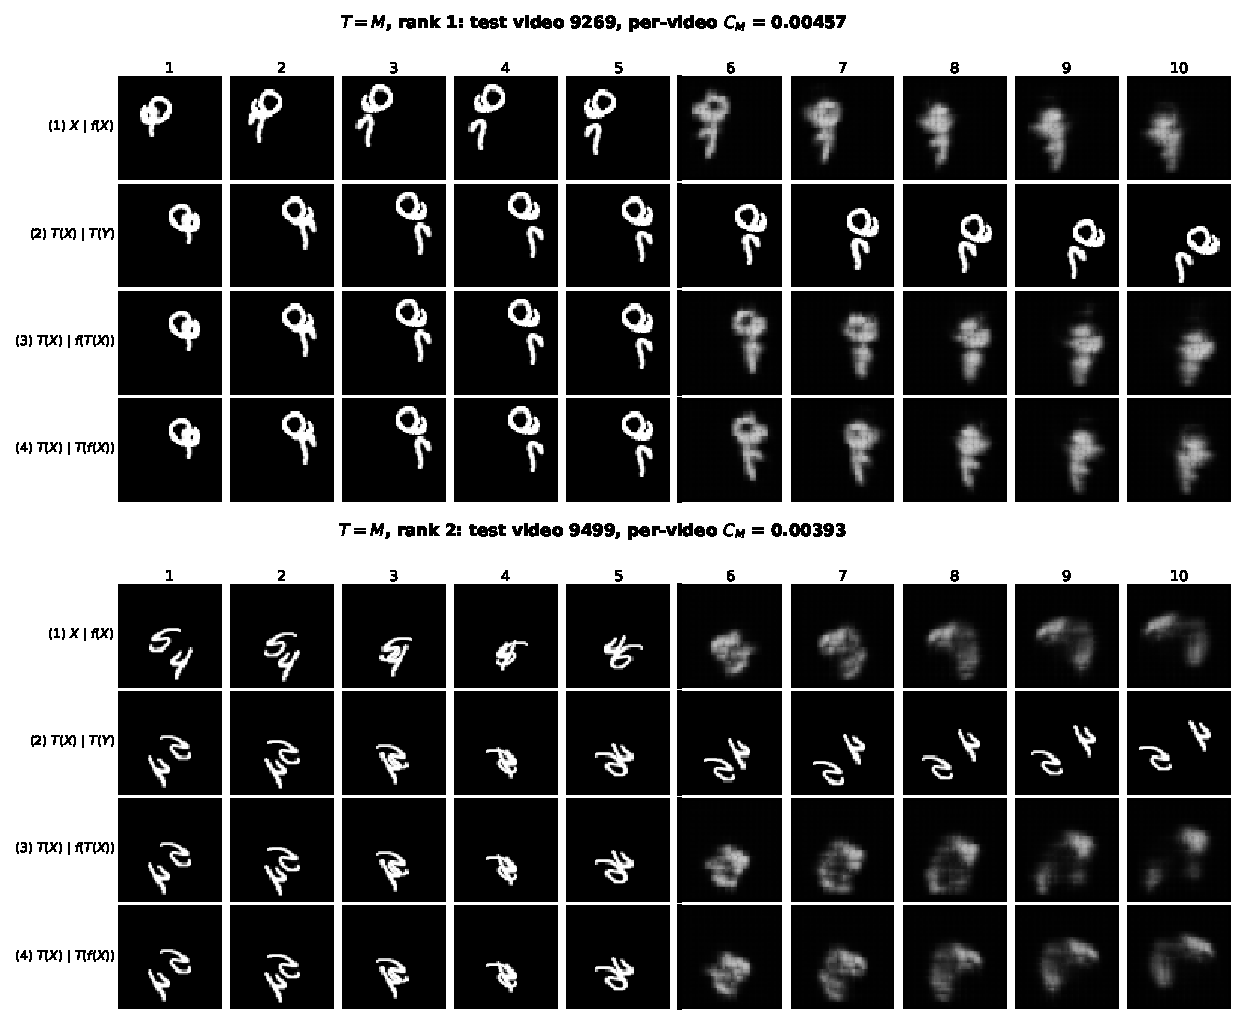
\includegraphics[width=0.8\linewidth]{fig3_M.pdf}\\[2pt]
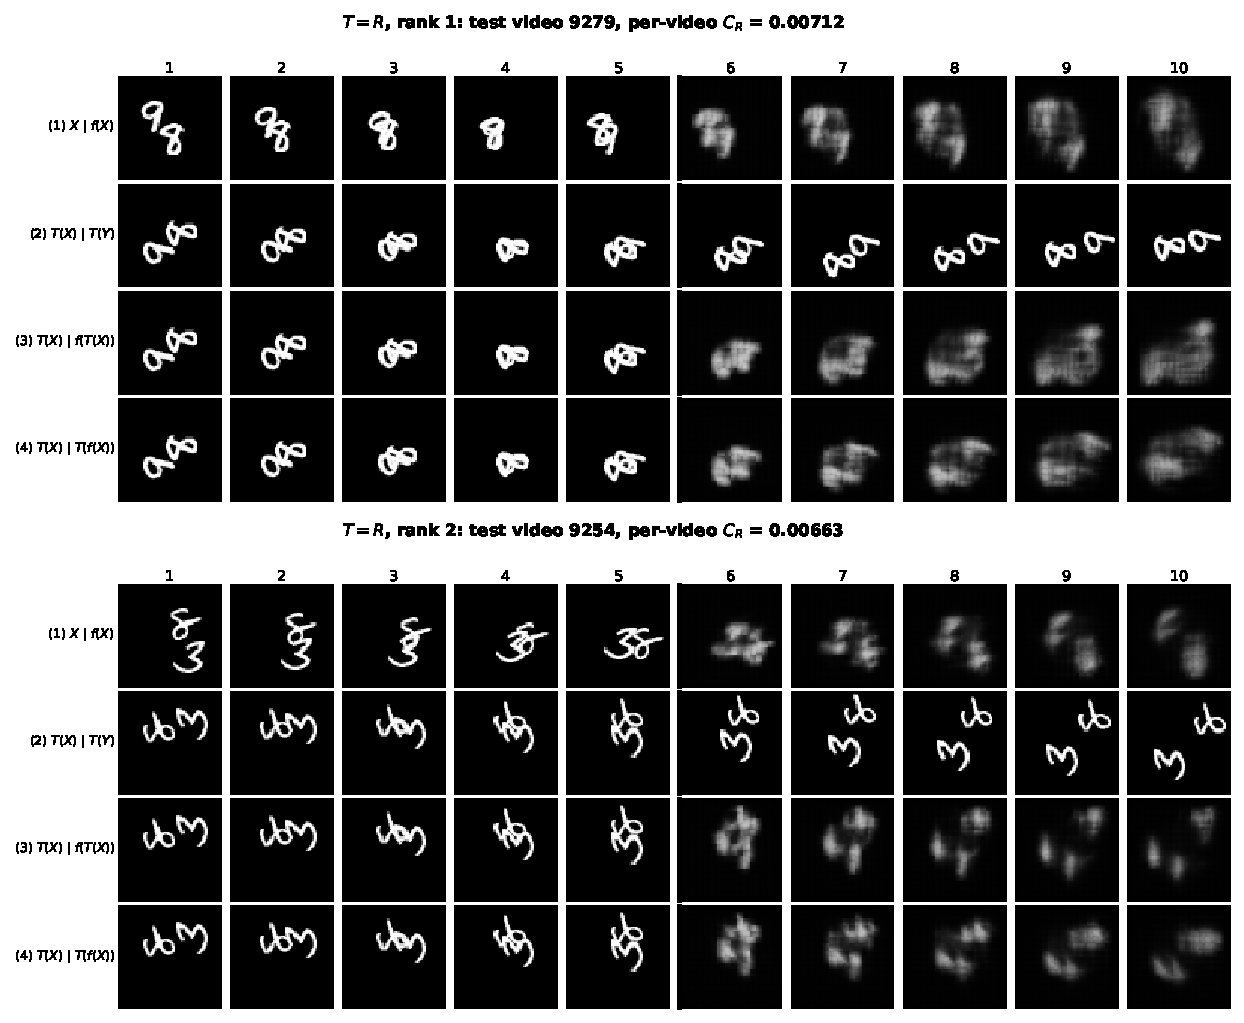
\includegraphics[width=0.8\linewidth]{fig3_R.pdf}
\caption{Model A (seed 0), $1\times$, $t=1$. Top: $T=M$, the two test videos with the largest per-video $C_M$ (9269, 9499); bottom: $T=R$, largest per-video $C_R$ (9279, 9254). Columns 1--5 are inputs, 6--10 the five future frames; rows (1) $X\,|\,f(X)$, (2) $T(X)\,|\,T(Y)$, (3) $T(X)\,|\,f(T(X))$, (4) $T(X)\,|\,T(f(X))$. Animated GIFs stepping through the five horizons with the same four rows (last input $|$ horizon $h$): \texttt{figures/gifs/fig3\_M\_rank1\_video9269.gif}, \texttt{fig3\_M\_rank2\_video9499.gif}, \texttt{fig3\_R\_rank1\_video9279.gif}, \texttt{fig3\_R\_rank2\_video9254.gif}.}\label{fig:f3}
\end{figure}
\begin{figure}[!htbp]\centering
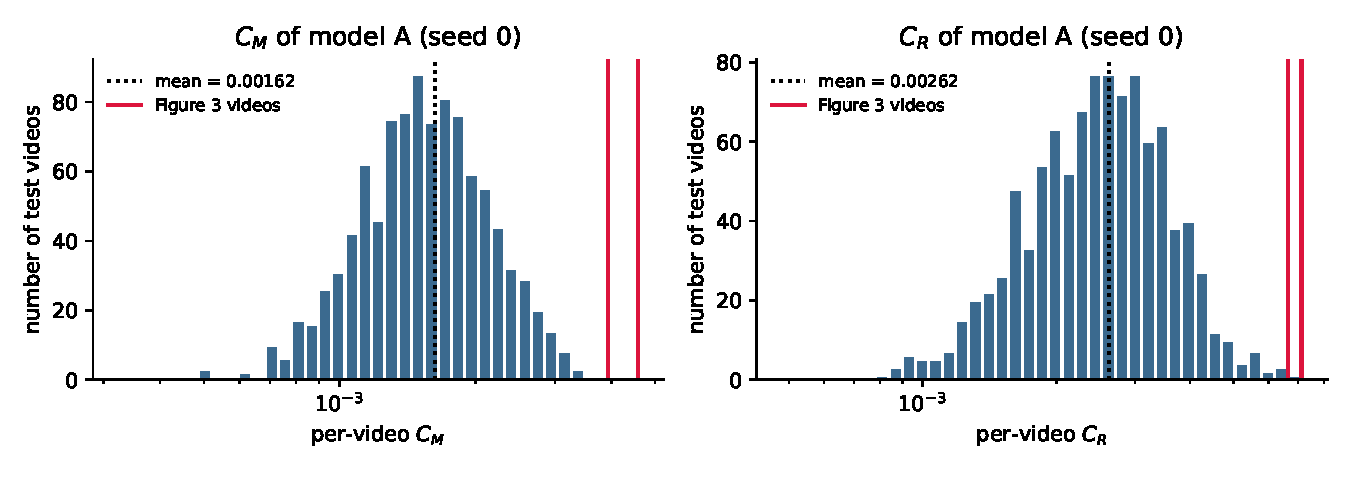
\includegraphics[width=0.85\linewidth]{fig4_hist.pdf}
\caption{Per-video $C_M$ (left) and $C_R$ (right) of model A (seed 0) over the 1000 test videos (log-scaled axis); red lines: the videos shown in Figure~\ref{fig:f3}; dotted: mean.}\label{fig:f4}
\end{figure}

\Q{Q2.6}{\textbf{Blank} (all zeros) and \textbf{Copy-last} are exactly consistent ($C_M=C_R=0$ in Table~\ref{tab:t3}) because both commute with every pixel permutation: $T(0)=0$, and copying the last frame commutes with mirroring or rotating it. So $C_T$ measures only whether the predictor treats a scene and its transformed copy \emph{alike}, never whether the prediction is \emph{right}: Blank is perfectly consistent and has $E^{(5)}=0.0426$, almost twice model A's. Consistency is necessary for a symmetric rule but not sufficient, and a blurrier forecast is more consistent almost by construction, so a small $C_T$ can come from vagueness. $E_T$, which compares the prediction for the transformed scene with the transformed truth, must always be read next to it. For model A: $C_M=0.00177$, $E_M=0.0226$ ($1.03\times E^{(5)}$), $C_R=0.00300$, $E_R=0.0237$ ($1.08\times$) --- consistent \emph{and} accurate, both far better than Copy-last ($0.0641$).}

\Q{Q2.7}{\textbf{Video 9279, $T=R$} (bottom of Figure~\ref{fig:f3}, rows 3 vs 4; seed-0 model A, $1\times$). Two digits (9 and 8) overlap in the last input frames and then separate. The truth (row 2) has its ink centroid moving $1.46$ px/frame. Row 4, $T(f(X))$ (original orientation), tracks it: centroid speed $1.44$ px/frame, the pair separates and drifts. Row 3, $f(T(X))$ (rotated input), \emph{stalls}: the centroid moves only $0.27$ px/frame (a fifth), ending $\approx5$\,px from where row 4 puts it, and the forecast becomes a horizontally smeared single blob whose total ink grows from $310$ ($h{=}1$) to $421$ ($h{=}5$) while the truth stays at $255$--$273$, and whose spread grows from $12.7$ to $18.0$ px (truth: $9.3\to12.4$). So the model's account changes from ``two digits that separate and move on'' to ``one digit-sized blob that stays put and blurs''. The other three videos disagree less: for $T=M$, video 9269, the two rows have the same centroid speed ($2.44$ vs $2.42$ px/frame against the true $3.29$) and differ mainly in blur details (centroid gap $1.5$ px).}

\Q{Q2.8}{\textbf{Yes, for model A rotation is harder than mirroring, and the difference comes from appearance, not motion.} Table~\ref{tab:t3}: $C_R=0.00300$ vs $C_M=0.00177$ ($1.7\times$) and $E_R-E^{(5)}=0.00174$ vs $E_M-E^{(5)}=0.00064$ ($2.7\times$). By Q2.1 neither transformation changes the motion statistics: directions are uniform and the speed is unchanged, so a purely motion-based rule would treat both alike. By Q2.2 both change the appearance, rotation more: $M$ flips the digits but keeps vertical strokes vertical and the stroke-orientation statistics roughly the same, whereas $R$ interchanges horizontal and vertical strokes, so rotated digits are further from anything seen in training. The part of the forecast that is carried by digit shape (keeping strokes sharp, resolving overlaps) is the part that degrades, as the stalled, blurred blob in Q2.7 shows. Model B (trained with $G$) tests this directly: if appearance is the cause, symmetry augmentation should shrink the gap (Table~\ref{tab:t5}). The gap itself is small compared with the speed failure below, so model A's motion rule is largely orientation-agnostic.}

\begin{table}[H]\centering\small
\caption{Speed test on the 1000 test videos ($t=1$). $E^{(2)}$ uses only the first two horizons (the only ones that exist at $3\times$).}\label{tab:t4}
\begin{tabular}{lrrrrr}\toprule
Predictor & $E^{(2)}$ 1$\times$ & $E^{(2)}$ 2$\times$ & $E^{(2)}$ 3$\times$ & $E^{(5)}$ 1$\times$ & $E^{(5)}$ 2$\times$ \\ \midrule
Model A (mean of seeds 0, 1) & 0.0187 & 0.0444 & 0.0516 & 0.0220 & 0.0492 \\
\quad seed 0 & 0.0189 & 0.0433 & 0.0508 & 0.0222 & 0.0477 \\
\quad seed 1 & 0.0185 & 0.0455 & 0.0524 & 0.0217 & 0.0507 \\
Copy-last & 0.0548 & 0.0661 & 0.0703 & 0.0641 & 0.0719 \\
Blank & 0.0426 & 0.0425 & 0.0426 & 0.0426 & 0.0425 \\
\bottomrule\end{tabular}
\end{table}
\begin{figure}[!htbp]\centering
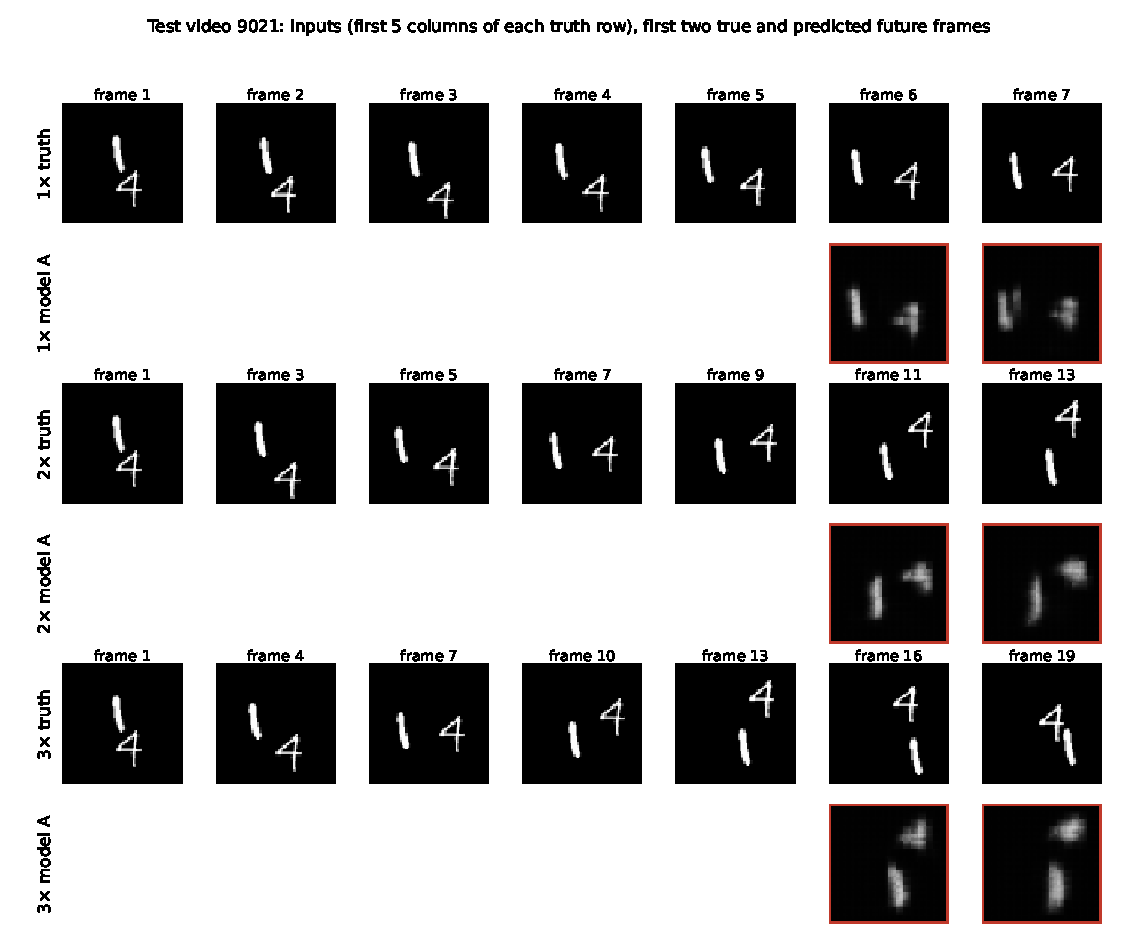
\includegraphics[width=0.93\linewidth]{fig5_speed.pdf}
\caption{Model A (seed 0), test video 9021 (digits do not overlap in any displayed true frame): five input frames, first two true future frames, and the first two predicted frames (red) at $1\times$, $2\times$, $3\times$ ($t=1$; frame numbers above each column).}\label{fig:f5}
\end{figure}

\Q{Q2.9}{\textbf{Where it falls apart.} $1\times$ is fine; at $2\times$ the error already jumps to $E^{(2)}=0.0444$ ($2.4\times$ its $1\times$ value $0.0187$; better than Copy-last $0.0661$ but \emph{worse} than Blank $0.0426$) and at $3\times$ it is $0.0516$ (Copy-last $0.0703$, Blank $0.0426$); the $E^{(5)}$ at $2\times$ is $0.0492$ against $0.0220$ at $1\times$. Table~S1 (row A, in Section 5) measures what goes wrong: from the last input frame to the first forecast, a digit's centroid truly moves $3.6$, $7.1$, $10.4$ px at $1\times$, $2\times$, $3\times$; model A moves its predicted digit by $3.3$--$3.4$ ($95\%$ of the truth), $2.5$ ($39\%$) and $1.8$--$2.3$ px ($19$--$25\%$). So \emph{it does not agree with my reach estimate}: with $8$\,px reach, $2\times$ (true displacement $7.1$\,px for the median digit, $<8$) should still work for most digits, yet the failure already starts there, and by $3\times$ ($10.4>8$) it is nearly total. What the estimate missed: the reach is a \emph{maximum} possible path, not what the network has learned to use. Trained only on displacements of about $3$--$4$\,px, the outer cells of its kernels (those that would carry a $7$\,px jump) have never been needed, so the effective reach is smaller than the nominal one, and $2\times$ is also simply unfamiliar. \textbf{What the failure looks like (Figure~\ref{fig:f5}):} \emph{stalling} and \emph{blur}: at $2\times$ and $3\times$ the digits appear washed out and close to the position where they were last seen, with a faint trailing smear toward the true position, but they do not move $k\times$ as far. I see no duplicated digit and no complete vanishing (intensity is lower but present). A stalled digit means the network failed to link the old position held in its state with the new position (it falls back on ``no motion''); a blur means it spreads probability over positions it cannot distinguish, as expected under squared error.}

\Q{Q2.10}{\textbf{No, not from these results alone.} Model A has a single training speed \emph{and} a single, small reach, so the two explanations predict the same thing, a failure at $2\times$ and $3\times$: ``fast motion never appeared in training'' and ``it is beyond the model's reach'' are confounded. The displacement numbers only hint: $2\times$ ($7.1$ px, below the nominal reach) fails, favouring unfamiliarity at least there, but the effective reach is unknown. \textbf{An experiment that separates them:} train the same architecture on all three speeds (model C: familiarity restored, reach unchanged) and a larger-reach architecture (model D) on the same data, and evaluate each at $2\times$ and $3\times$: if C fixes a speed, that failure was unfamiliar motion; if C still fails where D succeeds, it was reach. A cleaner variant is the \emph{reach-only} control, a larger-reach model trained at $1\times$ only: if it still fails at $2\times$, unfamiliarity is the cause, even though the displacement is now within reach.}
